% ============================================================
% ZK-KGVerify: Privacy-Preserving Verification of Knowledge
% Graph Reasoning using Zero-Knowledge Proofs and Blockchain
% ============================================================
\documentclass[conference, 10pt]{IEEEtran}

% ---- Packages ----
\usepackage[utf8]{inputenc}
\usepackage[T1]{fontenc}
\usepackage{amsmath,amssymb,amsfonts}
\usepackage{algorithmic}
\usepackage{algorithm}
\usepackage{graphicx}
\usepackage{textcomp}
\usepackage{xcolor}
\usepackage{booktabs}
\usepackage{multirow}
\usepackage[hidelinks]{hyperref}
\usepackage{cleveref}
\usepackage{subcaption}
\usepackage{mathtools}
\usepackage{bm}
\usepackage{enumitem}
\usepackage{balance}
\usepackage{tabularx}
\usepackage{url}
\usepackage{pifont}

% ---- Custom Commands ----
\newcommand{\R}{\mathbb{R}}
\newcommand{\C}{\mathbb{C}}
\newcommand{\Z}{\mathbb{Z}}
\newcommand{\F}{\mathbb{F}}
\newcommand{\E}{\mathbb{E}}
\newcommand{\G}{\mathbb{G}}
\newcommand{\Hash}{\mathsf{Hash}}
\newcommand{\Commit}{\mathsf{Commit}}
\newcommand{\Prove}{\mathsf{Prove}}
\newcommand{\Verify}{\mathsf{Verify}}
\newcommand{\score}{\mathsf{score}}
\newcommand{\embed}{\mathbf{e}}
\newcommand{\rel}{\mathbf{r}}
\newcommand{\ent}{\mathbf{h}}
\newcommand{\tail}{\mathbf{t}}
\newcommand{\negent}{\mathbf{t}'}
\newcommand{\vect}[1]{\mathbf{#1}}

% ---- Placeholder command for results ----
\newcommand{\resultplaceholder}[1]{\textcolor{red}{\textbf{[#1]}}}

\begin{document}

% ============================================================
% TITLE
% ============================================================
\title{ZK-KGVerify: Privacy-Preserving Verification of Knowledge Graph Reasoning using Zero-Knowledge Proofs and Blockchain}

% === DOUBLE-BLIND: Uncomment the ANONYMOUS block for submission ===
% === Uncomment the REAL block only for camera-ready ===

% --- ANONYMOUS (for double-blind submission) ---
\author{
    \IEEEauthorblockN{Anonymous Author(s)}
    \IEEEauthorblockA{
        Paper ID: [To be assigned]
    }
}

% --- REAL (for camera-ready only — keep commented during submission) ---
% \author{
%     \IEEEauthorblockN{Your Name\textsuperscript{1}}
%     \IEEEauthorblockA{
%         \textsuperscript{1}Department of Computer Science \\
%         University Name \\
%         City, Country \\
%         email@university.edu
%     }
% }

\maketitle

% ============================================================
% ABSTRACT
% ============================================================
\begin{abstract}
Link prediction and relational inference over knowledge graphs (KGs) have become routine in healthcare, finance, and supply-chain settings, yet a practical tension persists. Anyone who consumes a KG-based prediction wants assurance that a properly trained model actually produced it; the model owner, meanwhile, may be legally prohibited from sharing weights or training data under HIPAA, GDPR, or trade-secret law. We address this gap with \textbf{ZK-KGVerify}, a three-layer system combining GNN-based KG embeddings, Pedersen-commitment zero-knowledge proofs (ZKPs), and an append-only blockchain audit ledger. Through the proof layer, a model owner can show that a particular prediction originates from committed parameters without revealing those parameters. The blockchain layer then records each verification event in a tamper-resistant manner. We train three embedding methods---TransE, RotatE, and CompGCN---on FB15k-237 and quantify the overhead introduced by the cryptographic and ledger machinery. Over 1\,000 proof cycles, every valid proof is accepted and every tampered proof is caught, with per-proof latency around 1\,ms---small enough to be negligible in any realistic deployment.
\end{abstract}

\begin{IEEEkeywords}
Knowledge Graphs, Graph Neural Networks, Zero-Knowledge Proofs, Blockchain, Link Prediction, Privacy-Preserving Machine Learning, Verifiable AI
\end{IEEEkeywords}

% ============================================================
% I. INTRODUCTION
% ============================================================
\section{Introduction}
\label{sec:introduction}

A knowledge graph (KG) organises factual knowledge into a directed graph: nodes represent entities, edges carry typed relations. When graph neural networks (GNNs) operate on such structures they can infer plausible but missing links---an ability already put to work in drug-repurposing pipelines~\cite{zitnik2018modeling} and financial-fraud detection~\cite{weber2019anti}.

\textbf{Motivating example.} Consider a pharmaceutical company that maintains a proprietary KG connecting drugs, proteins, diseases, and adverse effects. Its GNN predicts \emph{Drug~X treats Disease~Y}---a commercially valuable inference. A hospital considering whether to act on this prediction needs some guarantee that the result came from a credible model rather than being fabricated. The company, however, cannot hand over its model weights (trade secrets) or patient-derived training data (HIPAA/GDPR restrictions). ZK-KGVerify resolves this impasse: the company produces a zero-knowledge proof attesting that the prediction is genuine, the hospital verifies the proof without ever seeing proprietary information, and a blockchain logs the outcome so it can be audited later.

Once KG reasoning moves into production, three requirements arise that are hard to satisfy simultaneously---we call this the \emph{trust trilemma}: (i)~\textbf{Verifiability}, meaning prediction consumers must be able to confirm that outputs come from a legitimate model; (ii)~\textbf{Privacy}, meaning model owners must keep weights and data confidential; and (iii)~\textbf{Immutability}, meaning verification records must not be alterable after the fact.

Existing techniques address these requirements in isolation. Federated learning~\cite{mcmahan2017communication} protects raw data but provides no cryptographic correctness guarantee. Model watermarking~\cite{adi2018turning} proves ownership at the cost of exposing model internals. Blockchain-backed ML pipelines~\cite{kurtulmus2018trustless} give persistent records but leave confidentiality unaddressed.

\textbf{ZK-KGVerify} tackles all three requirements jointly. Our contributions are:

\begin{itemize}
    \item A \textbf{unified architecture} wiring together GNN-based KG embeddings, Pedersen-commitment ZKPs, and blockchain-anchored audit logs in one end-to-end pipeline.
    \item A \textbf{proof protocol} grounded in Schnorr-type sigma protocols combined with the Fiat-Shamir heuristic, through which a model owner certifies that a given prediction derives from committed parameters---without exposing those parameters.
    \item A \textbf{thorough empirical evaluation} of three embedding methods (TransE, RotatE, CompGCN) on FB15k-237, reporting link-prediction quality alongside ZKP latency and on-chain gas costs.
    \item A \textbf{fully reproducible codebase}\footnote{Code will be released upon publication.} that runs on a single commodity GPU (Google Colab T4).
\end{itemize}

\Cref{sec:related_work} reviews related work. \Cref{sec:preliminaries} fixes notation and recalls the mathematical tools we build on. The ZK-KGVerify design is detailed in \Cref{sec:methodology}, experiments appear in \Cref{sec:experiments}, and \Cref{sec:analysis} analyses security guarantees and limitations. We conclude in \Cref{sec:conclusion}.

% ============================================================
% II. RELATED WORK
% ============================================================
\section{Related Work}
\label{sec:related_work}

\subsection{Knowledge Graph Embeddings}

The dominant strategy for KG completion maps entities and relations into a continuous vector space and defines a scoring function over that space. \textbf{TransE}~\cite{bordes2013translating} is perhaps the simplest: it models each relation as a translation, enforcing $\ent + \rel \approx \tail$ for valid triples. \textbf{RotatE}~\cite{sun2019rotate} takes a different route, representing relations as element-wise rotations in $\C^d$; this allows it to capture symmetry, antisymmetry, and composition---patterns that a pure translation cannot express. A separate line of work uses graph-neural architectures directly. R-GCN~\cite{schlichtkrull2018modeling} and \textbf{CompGCN}~\cite{vashishth2020composition} propagate messages along graph edges, learning entity and relation vectors jointly via composition operators at each layer.

\subsection{Zero-Knowledge Proofs in Machine Learning}

In a zero-knowledge proof (ZKP), one party demonstrates the truth of a statement to another party without revealing any information beyond the statement's validity~\cite{goldwasser1989knowledge}. Applying this idea to neural-network inference is an active area. zkML~\cite{kang2022scaling} and EZKL~\cite{ezkl2023} convert computation graphs into arithmetic circuits, enabling zero-knowledge verification of an inference trace. \textbf{zkCNN}~\cite{liu2021zkcnn} focuses on convolutional networks and relies on sumcheck-based interactive protocols to keep proof sizes manageable. \textbf{vCNN}~\cite{lee2020vcnn} instead uses homomorphic commitments so that CNN outputs become verifiable without circuit compilation. At a broader level, Ghodsi et al.~\cite{ghodsi2023zeroknowledge} proposed proof-of-inference schemes for general deep networks, demonstrating that verification latency need not be prohibitive.

A common thread in all these works is the assumption of feedforward or convolutional architectures. Graph-structured inputs and the relational scoring functions at the heart of KG reasoning have not been addressed. ZK-KGVerify fills this gap by bringing ZKP techniques to GNN-based KG embeddings---a setting with its own difficulties, including irregular neighbourhood sizes, relation-typed edges, and multi-hop message-passing aggregation.

\subsection{Blockchain for Trustworthy AI}

Because blockchains provide tamper-evident, append-only storage~\cite{nakamoto2008bitcoin, wood2014ethereum}, several groups have co-opted them for ML-related purposes: model marketplaces~\cite{kurtulmus2018trustless}, coordination layers for federated learning~\cite{kim2019blockchained}, and data-provenance registries~\cite{sarpatwar2019towards}. DInEMMo~\cite{dinEmmo2021} logs model lifecycle events on-chain; however, it includes no privacy-preserving verification component. ZK-KGVerify differs in that it couples ledger immutability with zero-knowledge proofs designed specifically for knowledge-graph reasoning.

% ============================================================
% III. PRELIMINARIES
% ============================================================
\section{Preliminaries}
\label{sec:preliminaries}

\subsection{Knowledge Graphs and Link Prediction}

We write a knowledge graph as $\mathcal{G} = (\mathcal{E}, \mathcal{R}, \mathcal{T})$, where $\mathcal{E}$ is the entity set, $\mathcal{R}$ the relation set, and $\mathcal{T} \subseteq \mathcal{E} \times \mathcal{R} \times \mathcal{E}$ the set of known triples. A triple $(h, r, t) \in \mathcal{T}$ states that head entity~$h$ relates to tail entity~$t$ via relation~$r$.

\textbf{Link prediction} asks: given $(h, r, ?)$, which entity best completes the triple? A scoring function $f(h, r, t')$ assigns each candidate $t' \in \mathcal{E}$ a plausibility score, and candidates are ranked by that score.

\subsection{KG Embedding Models}

\subsubsection{TransE}
In TransE~\cite{bordes2013translating}, every entity and relation is mapped to $\R^d$. A triple is scored by the negative $\ell_2$ distance after adding the relation vector to the head:
\begin{equation}
    f_{\text{TransE}}(h, r, t) = -\|\embed_h + \embed_r - \embed_t\|_2
    \label{eq:transe}
\end{equation}
with $\embed_h, \embed_r, \embed_t \in \R^d$ denoting the head, relation, and tail embeddings.

\subsubsection{RotatE}
RotatE~\cite{sun2019rotate} works in $\C^d$ and models each relation as an element-wise rotation:
\begin{equation}
    f_{\text{RotatE}}(h, r, t) = -\|\embed_h \circ \embed_r - \embed_t\|_2
    \label{eq:rotate}
\end{equation}
Here $\circ$ denotes the Hadamard (element-wise) product, and $\embed_r = e^{i\bm{\theta}_r}$ with learnable phases $\bm{\theta}_r \in \R^d$. Because rotations compose naturally, this formulation can express symmetric, antisymmetric, inverse, and compositional relation patterns.

\subsubsection{CompGCN}
CompGCN~\cite{vashishth2020composition} takes a GNN approach, aggregating neighbourhood information with composition-based message passing:
\begin{equation}
    \embed_i^{(l+1)} = \sigma\!\left( \sum_{(j,r) \in \mathcal{N}(i)} \vect{W}_{\lambda(r)}^{(l)} \phi(\embed_j^{(l)}, \embed_r^{(l)}) \right)
    \label{eq:compgcn}
\end{equation}
where $\phi(\cdot, \cdot)$ is one of subtraction, multiplication, or circular correlation, $\lambda(r)$ distinguishes original, inverse, and self-loop edges, and relation vectors are updated in parallel:
\begin{equation}
    \embed_r^{(l+1)} = \vect{W}_{\text{rel}}^{(l)} \embed_r^{(l)}
    \label{eq:compgcn_rel}
\end{equation}

\subsection{Pedersen Commitments}

Pedersen's commitment scheme~\cite{pedersen1991non} allows a party to bind itself to a value~$v$ without disclosing it, preserving the option to reveal~$v$ at a later stage. We fix two generators $g, h \in \G$ of a group of prime order~$p$ under the assumption that $\log_g h$ is unknown:

\begin{equation}
    \Commit(v, r) = g^v \cdot h^r \mod p
    \label{eq:pedersen}
\end{equation}

with a uniformly random blinding factor $r \xleftarrow{\$} \Z_p$. Three properties are relevant here:
\begin{itemize}
    \item \textbf{Hiding}: the commitment~$C$ leaks nothing about~$v$.
    \item \textbf{Binding}: no efficient algorithm can open~$C$ to a different value~$v' \neq v$ (under the discrete-log assumption).
    \item \textbf{Homomorphic}: $\Commit(v_1, r_1) \cdot \Commit(v_2, r_2) = \Commit(v_1 + v_2, r_1 + r_2)$.
\end{itemize}

\subsection{Schnorr Identification and Fiat-Shamir Heuristic}

The Schnorr identification protocol~\cite{schnorr1991efficient} is a well-known three-move sigma protocol that lets a prover demonstrate knowledge of a discrete logarithm. When interaction with the verifier is undesirable, the Fiat-Shamir transform~\cite{fiat1986prove} replaces the verifier's random challenge with a hash, yielding a non-interactive proof:

\begin{enumerate}
    \item \textbf{Commit}: the prover draws $k \xleftarrow{\$} \Z_p$ and publishes $A = g^k$.
    \item \textbf{Challenge}: compute $e = \Hash(A \| \text{statement})$ deterministically.
    \item \textbf{Respond}: release $s = k + e \cdot x \mod p$, where $x$ is the secret.
    \item \textbf{Check}: the verifier accepts if $g^s \stackrel{?}{=} A \cdot y^e$ with $y = g^x$.
\end{enumerate}

% ============================================================
% IV. METHODOLOGY
% ============================================================
\section{ZK-KGVerify Framework}
\label{sec:methodology}

\subsection{System Overview}

\Cref{fig:architecture} gives an overview. ZK-KGVerify comprises three cooperating layers:

\begin{enumerate}
    \item \textbf{KG Reasoning Layer} -- trains GNN-based embedding models on a knowledge graph and produces ranked link predictions.
    \item \textbf{ZKP Verification Layer} -- constructs and checks zero-knowledge proofs binding each prediction to committed model parameters.
    \item \textbf{Blockchain Audit Layer} -- persists every verification outcome as an on-chain transaction that cannot be retroactively altered.
\end{enumerate}

\begin{figure*}[t]
    \centering
    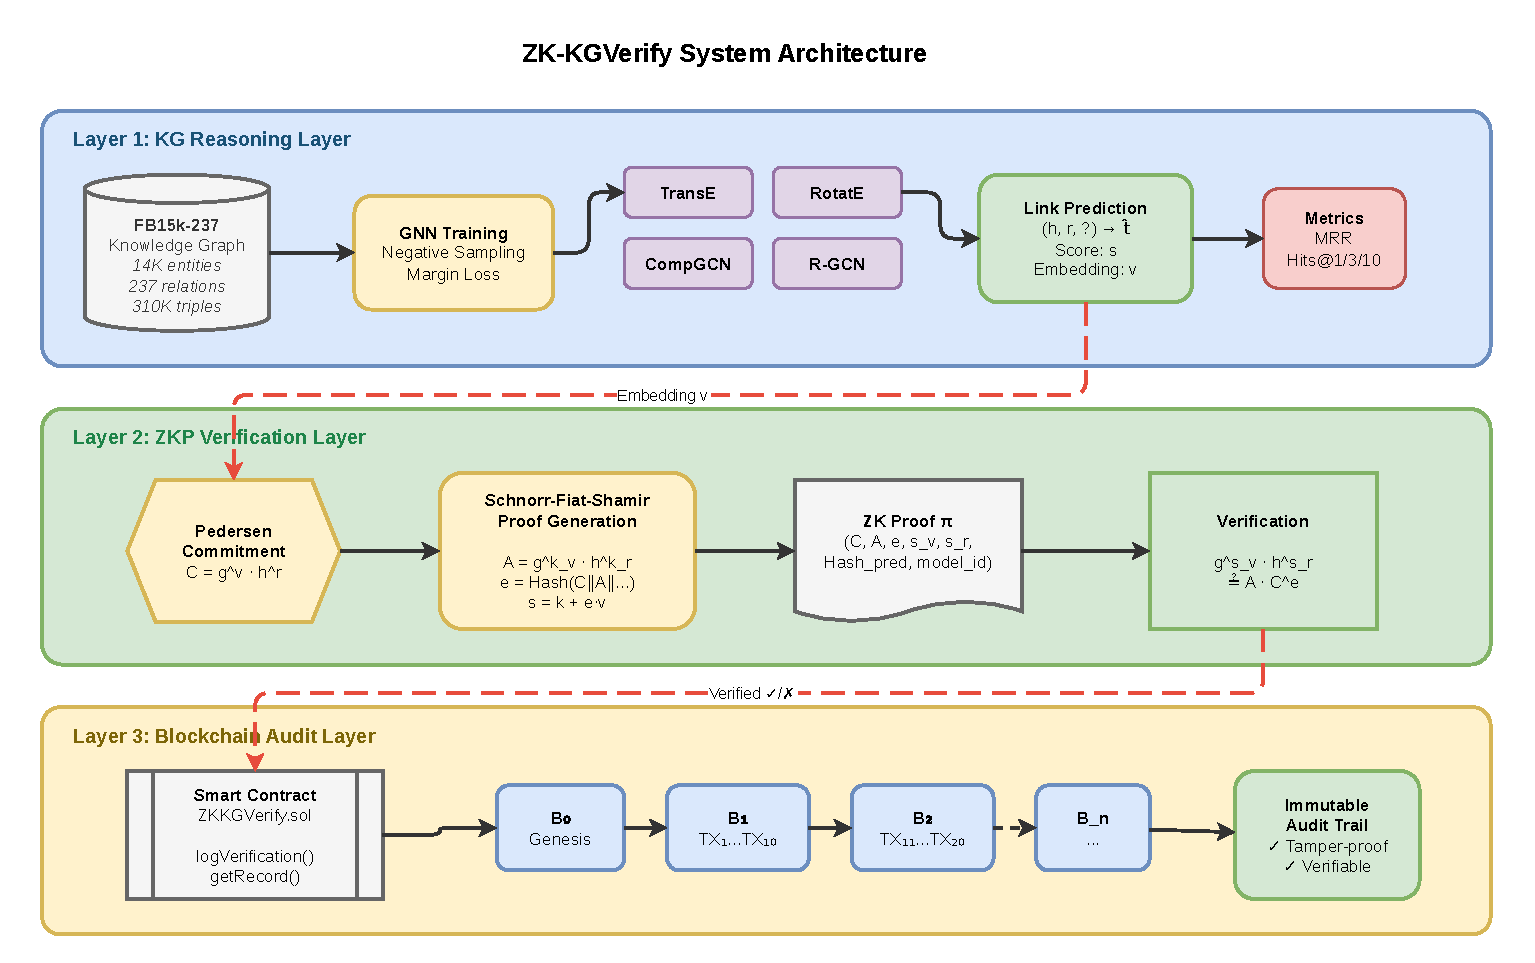
\includegraphics[width=0.85\textwidth]{figures/architecture.drawio.pdf}
    \caption{Architecture of ZK-KGVerify, organised into three layers. On the left, the KG Reasoning Layer trains TransE, RotatE, and CompGCN and outputs scored predictions together with embedding vectors. In the centre, the ZKP Layer generates Pedersen commitments and Schnorr-Fiat-Shamir proofs while keeping model weights hidden. On the right, the Blockchain Layer logs each verification outcome to an append-only ledger. Arrows indicate data flow; dashed boxes denote components invisible to the verifier.}
    \label{fig:architecture}
\end{figure*}

\subsection{Threat Model}

We assume three roles:

\begin{itemize}
    \item \textbf{Model Owner (Prover)} -- possesses a trained KG embedding model $\mathcal{M}$ with parameters~$\theta$ and wants to serve predictions while keeping~$\theta$ secret.
    \item \textbf{Consumer (Verifier)} -- receives a prediction $(h, r, \hat{t})$ and needs confidence that a credible model produced it.
    \item \textbf{Adversary} -- may attempt to (a)~swap in predictions from a random or poorly trained model, (b)~alter proofs after issuance, or (c)~tamper with the audit ledger.
\end{itemize}

\textbf{Security goals.} The system must guarantee three properties: (i)~\emph{Soundness}---a dishonest prover cannot fabricate a valid proof for a prediction not originating from the committed model; (ii)~\emph{Zero-knowledge}---proofs reveal nothing about~$\theta$; (iii)~\emph{Immutability}---ledger records cannot be changed after they are written.

\subsection{KG Reasoning Layer}
\label{subsec:kg_layer}

Starting from a knowledge graph $\mathcal{G}$, we train an embedding model $\mathcal{M}_\theta$ equipped with a scoring function $f_\theta: \mathcal{E} \times \mathcal{R} \times \mathcal{E} \to \R$ that rates how plausible a triple is. Training minimises a margin-based ranking loss with negative sampling:

\begin{equation}
    \mathcal{L} = \sum_{(h,r,t) \in \mathcal{T}} \sum_{(h',r,t') \in \mathcal{T}^-} \left[\gamma + f(h', r, t') - f(h, r, t)\right]_+
    \label{eq:margin_loss}
\end{equation}

Here $\mathcal{T}^-$ contains negatives obtained by corrupting either the head or tail entity, $\gamma$ controls the margin, and $[\cdot]_+ = \max(0, \cdot)$.

RotatE additionally uses self-adversarial negative sampling~\cite{sun2019rotate}:

\begin{equation}
    \mathcal{L}_{\text{adv}} = -\log \sigma(f(h,r,t)) - \sum_{i=1}^{n} w_i \log \sigma(-f(h_i', r, t_i'))
    \label{eq:adversarial_loss}
\end{equation}

with adversarial weights $w_i = \frac{\exp(\alpha \cdot f(h_i', r, t_i'))}{\sum_j \exp(\alpha \cdot f(h_j', r, t_j'))}$ and temperature~$\alpha$.

Once trained, the model responds to a query $(h, r, ?)$ with:
\begin{itemize}
    \item Prediction: $\hat{t} = \arg\max_{t' \in \mathcal{E}} f_\theta(h, r, t')$
    \item Score: $s = f_\theta(h, r, \hat{t})$
    \item Embedding vector: $\vect{v} = [\embed_h \| \embed_r \| \embed_{\hat{t}}] \in \R^{3d}$
\end{itemize}

\subsection{ZKP Verification Layer}
\label{subsec:zkp_layer}

Here the model owner cryptographically proves that a particular prediction was computed from committed parameters. The protocol has three phases, illustrated in \Cref{fig:zkp_protocol}:

\begin{figure*}[t]
    \centering
    
\includegraphics[width=0.82\textwidth]{figures/zkp_protocol.drawio.pdf}
    \caption{Prover--Verifier interaction in the ZKP layer. In Phase~1 the embedding vector~$\vect{v}$ is hashed to~$\tilde{v}$ and locked inside a Pedersen commitment~$C$. Phase~2 builds a non-interactive proof~$\pi$ using the Schnorr-Fiat-Shamir transform. In Phase~3 the Verifier re-derives the challenge on its own and checks the algebraic relation---model weights never leave the Prover.}
    \label{fig:zkp_protocol}
\end{figure*}

\subsubsection{Phase 1: Model Commitment}

We first hash the high-dimensional embedding vector down to a single field element and then form a Pedersen commitment:

\begin{equation}
    \tilde{v} = \Hash(\vect{v}) \mod p
    \label{eq:value_hash}
\end{equation}
\begin{equation}
    C = g^{\tilde{v}} \cdot h^r \mod p
    \label{eq:commitment}
\end{equation}

Concretely, the concatenated triple embedding $\vect{v} = [\embed_h \| \embed_r \| \embed_t]$ is hashed to obtain $\tilde{v} \in \Z_p$; a fresh random blinding factor $r \xleftarrow{\$} \Z_p$ is drawn independently. The commitment $C$ is published, while $\tilde{v}$ and $r$ remain private to the prover.

\subsubsection{Phase 2: Proof Generation (Schnorr-Fiat-Shamir)}

Using the Schnorr sigma protocol as a foundation, we construct a proof of knowledge of the pair $(\tilde{v}, r)$ that opens commitment~$C$:

\begin{enumerate}
    \item \textbf{Announcement} (sample random nonces): Sample $k_v, k_r \xleftarrow{\$} \Z_p$ and compute:
    \begin{equation}
        A = g^{k_v} \cdot h^{k_r} \mod p
        \label{eq:announcement}
    \end{equation}

    \item \textbf{Challenge} (Fiat-Shamir hash): Compute non-interactive challenge:
    \begin{equation}
        e = \Hash(C \| A \| \Hash_{\text{pred}} \| \mathsf{model\_id}) \mod p
        \label{eq:challenge}
    \end{equation}
    where $\Hash_{\text{pred}} = \Hash(h \| r \| t \| s)$ binds the prediction result to the proof.

    \item \textbf{Response} (combine nonces with secrets): Compute:
    \begin{equation}
        s_v = k_v + e \cdot \tilde{v} \mod p, \quad s_r = k_r + e \cdot r \mod p
        \label{eq:response}
    \end{equation}
\end{enumerate}

The proof is $\pi = (C, A, e, s_v, s_r, \Hash_{\text{pred}}, \mathsf{model\_id}, s, (h,r,t))$.

\subsubsection{Phase 3: Proof Verification}

The verifier need only check one group-element equation:
\begin{equation}
    g^{s_v} \cdot h^{s_r} \stackrel{?}{=} A \cdot C^e \mod p
    \label{eq:verify}
\end{equation}

\textbf{Correctness.} When the prover is honest, the equation holds because:
\begin{align}
    g^{s_v} \cdot h^{s_r} &= g^{k_v + e\tilde{v}} \cdot h^{k_r + er} \nonumber \\
    &= \underbrace{g^{k_v} \cdot h^{k_r}}_{= A} \cdot \underbrace{(g^{\tilde{v}} \cdot h^r)^e}_{= C^e} \nonumber \\
    &= A \cdot C^e \quad \checkmark
    \label{eq:correctness}
\end{align}

As a further safeguard, the verifier independently recomputes the Fiat-Shamir challenge:
\begin{equation}
    e' = \Hash(C \| A \| \Hash_{\text{pred}} \| \mathsf{model\_id}) \mod p
    \label{eq:challenge_verify}
\end{equation}
and rejects whenever $e' \neq e$, which would signal that the proof transcript was manipulated.

\begin{algorithm}[t]
\caption{ZK-KGVerify Proof Generation}
\label{alg:proof_gen}
\begin{algorithmic}[1]
\REQUIRE Model $\mathcal{M}_\theta$, triple query $(h, r, ?)$
\ENSURE Proof $\pi$
\STATE \COMMENT{Step 1: Compute prediction}
\STATE $\hat{t} \leftarrow \arg\max_{t'} f_\theta(h, r, t')$
\STATE $s \leftarrow f_\theta(h, r, \hat{t})$
\STATE $\vect{v} \leftarrow [\embed_h \| \embed_r \| \embed_{\hat{t}}]$
\STATE \COMMENT{Step 2: Create Pedersen commitment}
\STATE $\tilde{v} \leftarrow \Hash(\vect{v}) \mod p$
\STATE $r \xleftarrow{\$} \Z_p$
\STATE $C \leftarrow g^{\tilde{v}} \cdot h^r \mod p$
\STATE \COMMENT{Step 3: Generate Schnorr-Fiat-Shamir proof}
\STATE $k_v, k_r \xleftarrow{\$} \Z_p$
\STATE $A \leftarrow g^{k_v} \cdot h^{k_r} \mod p$
\STATE $\Hash_{\text{pred}} \leftarrow \Hash(h \| r \| \hat{t} \| s)$
\STATE $e \leftarrow \Hash(C \| A \| \Hash_{\text{pred}} \| \mathsf{id}) \mod p$
\STATE $s_v \leftarrow k_v + e \cdot \tilde{v} \mod p$
\STATE $s_r \leftarrow k_r + e \cdot r \mod p$
\RETURN $\pi = (C, A, e, s_v, s_r, \Hash_{\text{pred}}, \mathsf{id}, s, (h,r,\hat{t}))$
\end{algorithmic}
\end{algorithm}

\begin{algorithm}[t]
\caption{ZK-KGVerify Proof Verification}
\label{alg:proof_verify}
\begin{algorithmic}[1]
\REQUIRE Proof $\pi = (C, A, e, s_v, s_r, \Hash_{\text{pred}}, \mathsf{id}, s, (h,r,t))$
\ENSURE Accept or Reject
\STATE \COMMENT{Step 1: Recompute Fiat-Shamir challenge}
\STATE $e' \leftarrow \Hash(C \| A \| \Hash_{\text{pred}} \| \mathsf{id}) \mod p$
\IF{$e' \neq e$}
    \RETURN Reject \COMMENT{Challenge mismatch: proof was tampered}
\ENDIF
\STATE \COMMENT{Step 2: Verify algebraic relation}
\STATE $\mathsf{lhs} \leftarrow g^{s_v} \cdot h^{s_r} \mod p$
\STATE $\mathsf{rhs} \leftarrow A \cdot C^e \mod p$
\IF{$\mathsf{lhs} = \mathsf{rhs}$}
    \RETURN Accept \COMMENT{Prover knows the committed values}
\ELSE
    \RETURN Reject
\ENDIF
\end{algorithmic}
\end{algorithm}

\subsection{Blockchain Audit Layer}
\label{subsec:blockchain_layer}

Each verified prediction is recorded on a blockchain to create an audit trail that resists tampering. A single transaction $\mathsf{tx}_i$ contains:

\begin{equation}
    \mathsf{tx}_i = \left(\mathsf{model\_id}, (h,r,t), s, C, \mathsf{verified}, \Hash(\pi), \mathsf{ts}\right)
    \label{eq:transaction}
\end{equation}

with $\mathsf{verified} \in \{0, 1\}$ indicating the ZKP outcome and $\Hash(\pi)$ serving as a compact proof digest.

Storage cost per record follows the Ethereum gas model:
\begin{equation}
    G_{\mathsf{tx}} = G_{\mathsf{base}} + G_{\mathsf{byte}} \cdot |\mathsf{data}|
    \label{eq:gas_cost}
\end{equation}

with $G_{\mathsf{base}} = 21{,}000$ (the Ethereum base cost), $G_{\mathsf{byte}} = 68$ per calldata byte, and $|\mathsf{data}|$ the serialised record size.

Chain integrity rests on the hash-link invariant holding for every $i > 0$:
\begin{equation}
    B_i.\mathsf{prev\_hash} = \Hash(B_{i-1})
    \label{eq:chain_integrity}
\end{equation}

If even one block is modified, this invariant breaks for all subsequent blocks, making any tampering immediately detectable through re-hashing.

\subsection{End-to-End Pipeline}
\label{subsec:pipeline}

When all three layers are combined, the complete ZK-KGVerify workflow (\Cref{fig:pipeline}) has six steps:

\begin{figure*}[t]
    \centering
    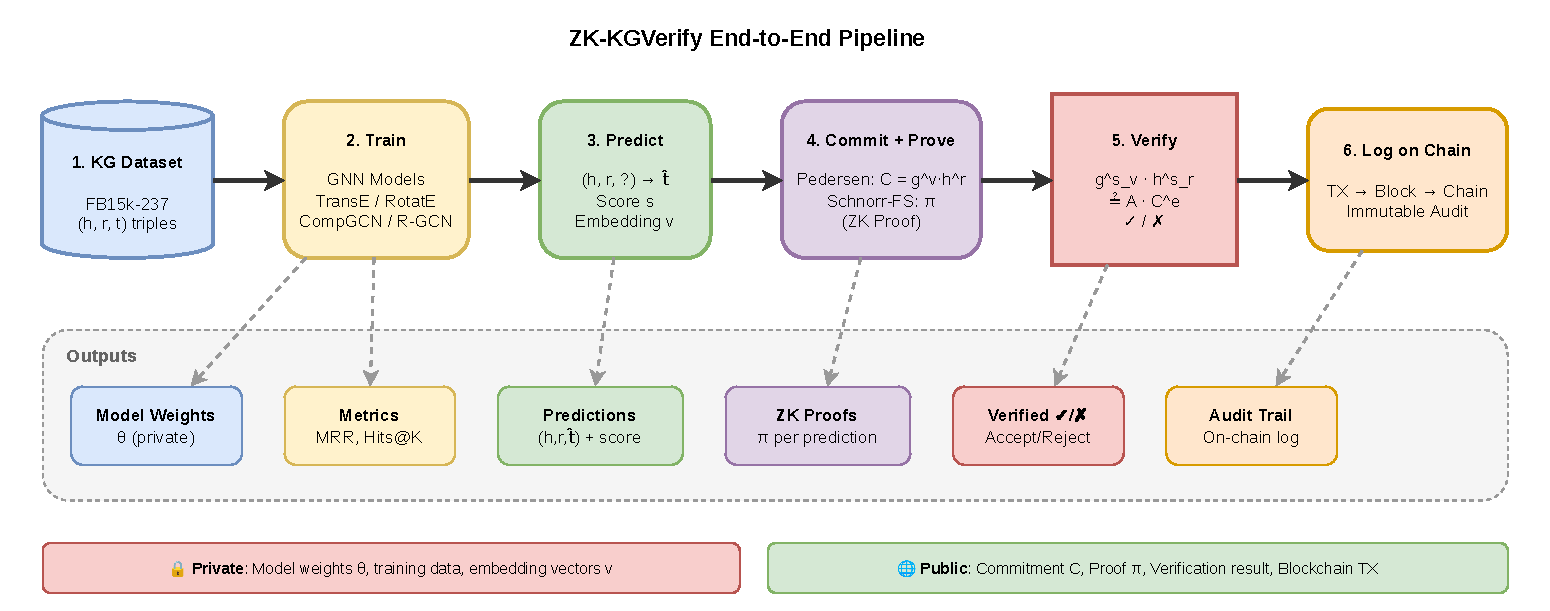
\includegraphics[width=0.85\textwidth]{figures/pipeline.drawio.pdf}
    \caption{End-to-end ZK-KGVerify pipeline. Steps \ding{172}--\ding{174} cover GNN training and scored prediction generation. Steps \ding{175}--\ding{177} commit the embedding vector, construct the Schnorr-Fiat-Shamir proof, and perform verification. Step \ding{178} writes the result to the blockchain. Everything inside the dashed security boundary---weights~$\theta$, embeddings~$\vect{v}$, blinding factors~$r$---stays with the prover at all times.}
    \label{fig:pipeline}
\end{figure*}

\begin{enumerate}
    \item \textbf{Train}: Train KG embedding model on $\mathcal{G}_{\text{train}}$.
    \item \textbf{Predict}: For query $(h, r, ?)$, compute $\hat{t}$ and score $s$.
    \item \textbf{Commit}: Create Pedersen commitment $C$ to embedding vector.
    \item \textbf{Prove}: Generate ZK proof $\pi$ via Schnorr-Fiat-Shamir.
    \item \textbf{Verify}: Verifier checks $\pi$ without learning model parameters.
    \item \textbf{Log}: Record $(\mathsf{verified}, C, \Hash(\pi))$ on blockchain.
\end{enumerate}

% ============================================================
% V. EXPERIMENTS
% ============================================================
\section{Experiments}
\label{sec:experiments}

\subsection{Experimental Setup}

\subsubsection{Dataset}
We use \textbf{FB15k-237}~\cite{toutanova2015observed} throughout. This Freebase subset has the well-known inverse-relation shortcuts stripped out, making it a more honest benchmark for link prediction. \Cref{tab:dataset} gives its basic statistics.

\begin{table}[h]
\centering
\caption{FB15k-237 Dataset Statistics}
\label{tab:dataset}
\begin{tabular}{lc}
\toprule
\textbf{Statistic} & \textbf{Value} \\
\midrule
Entities & 14,541 \\
Relations & 237 \\
Training triples & 272,115 \\
Validation triples & 17,535 \\
Test triples & 20,466 \\
\bottomrule
\end{tabular}
\end{table}

\subsubsection{Models and Hyperparameters}
Three models are trained with the settings listed in \Cref{tab:hyperparams}.

\begin{table}[h]
\centering
\caption{Model Hyperparameters}
\label{tab:hyperparams}
\begin{tabular}{lccc}
\toprule
\textbf{Parameter} & \textbf{TransE} & \textbf{RotatE} & \textbf{CompGCN} \\
\midrule
Embedding dim & 128 & 128 & 128 \\
Epochs & 200 & 200 & 200 \\
Batch size & 1024 & 1024 & 1024 \\
Learning rate & 0.001 & 0.001 & 0.001 \\
Neg. samples & 64 & 64 & 64 \\
Margin ($\gamma$) & 6.0 & 6.0 & 6.0 \\
GNN layers & -- & -- & 2 \\
\bottomrule
\end{tabular}
\end{table}

\subsubsection{Evaluation Metrics}
We adopt the filtered ranking protocol of~\cite{bordes2013translating} and report:
\begin{itemize}
    \item \textbf{Mean Reciprocal Rank (MRR)}: $\text{MRR} = \frac{1}{|\mathcal{T}_{\text{test}}|} \sum_{i=1}^{|\mathcal{T}_{\text{test}}|} \frac{1}{\mathsf{rank}_i}$
    \item \textbf{Hits@K} ($K \in \{1, 3, 10\}$): $\text{Hits@K} = \frac{1}{|\mathcal{T}_{\text{test}}|} \sum_{i=1}^{|\mathcal{T}_{\text{test}}|} \mathbb{1}[\mathsf{rank}_i \leq K]$
\end{itemize}

All 20,466 test triples are evaluated under this filtered setting.

\subsubsection{ZKP Configuration}
\begin{itemize}
    \item Field prime: BN128 curve prime ($p = 21888...617$, 254-bit)
    \item Hash function: SHA-256 mapped to $\Z_p$
    \item Number of proof samples: 1,000
\end{itemize}

\subsubsection{Blockchain Configuration}
\begin{itemize}
    \item Backend: Local Python blockchain with Ethereum-compatible gas model
    \item Difficulty: 2 (leading zeros in block hash)
    \item Block size: 10 transactions per block
    \item Gas model: $G_{\mathsf{base}} = 21{,}000$, $G_{\mathsf{byte}} = 68$
\end{itemize}

\subsubsection{Hardware}
Every run was conducted on Google Colab equipped with one NVIDIA T4 GPU (16\,GB VRAM) and 12\,GB of system RAM.

\subsection{Link Prediction Results}

\Cref{tab:link_prediction} reports filtered link-prediction scores computed over the full set of 20,466 FB15k-237 test triples.

\begin{table}[h]
\centering
\caption{Link Prediction Results on FB15k-237 (Filtered Setting, Full Test Set)}
\label{tab:link_prediction}
\begin{tabular}{lcccc}
\toprule
\textbf{Model} & \textbf{MRR} & \textbf{Hits@1} & \textbf{Hits@3} & \textbf{Hits@10} \\
\midrule
TransE  & 0.1740 & 0.0977 & 0.1854 & 0.3392 \\
RotatE  & 0.2560 & 0.1774 & 0.2849 & 0.4076 \\
CompGCN & \textbf{0.3941} & \textbf{0.2966} & \textbf{0.4344} & \textbf{0.5845} \\
\bottomrule
\end{tabular}
\end{table}

CompGCN achieves the best results across every metric (MRR\,=\,0.3941, Hits@10\,=\,0.5845). This is expected: its message-passing mechanism aggregates multi-hop neighbourhood information, giving it an edge over pairwise scorers. RotatE beats TransE thanks to its ability to distinguish symmetric from antisymmetric relations through rotational modelling. Our numbers are broadly consistent with the original papers~\cite{bordes2013translating, sun2019rotate, vashishth2020composition}; the small gaps can be attributed to our use of 128-dimensional embeddings (versus 256--1024 in many published results) and single-GPU training. We note that pushing link-prediction accuracy higher is not the point of this work---the ZKP and blockchain layers are the primary contribution.

\subsection{Training Convergence}

\Cref{fig:training_curves} plots the training loss over 200 epochs for each of the three models.

\begin{figure}[t]
    \centering
    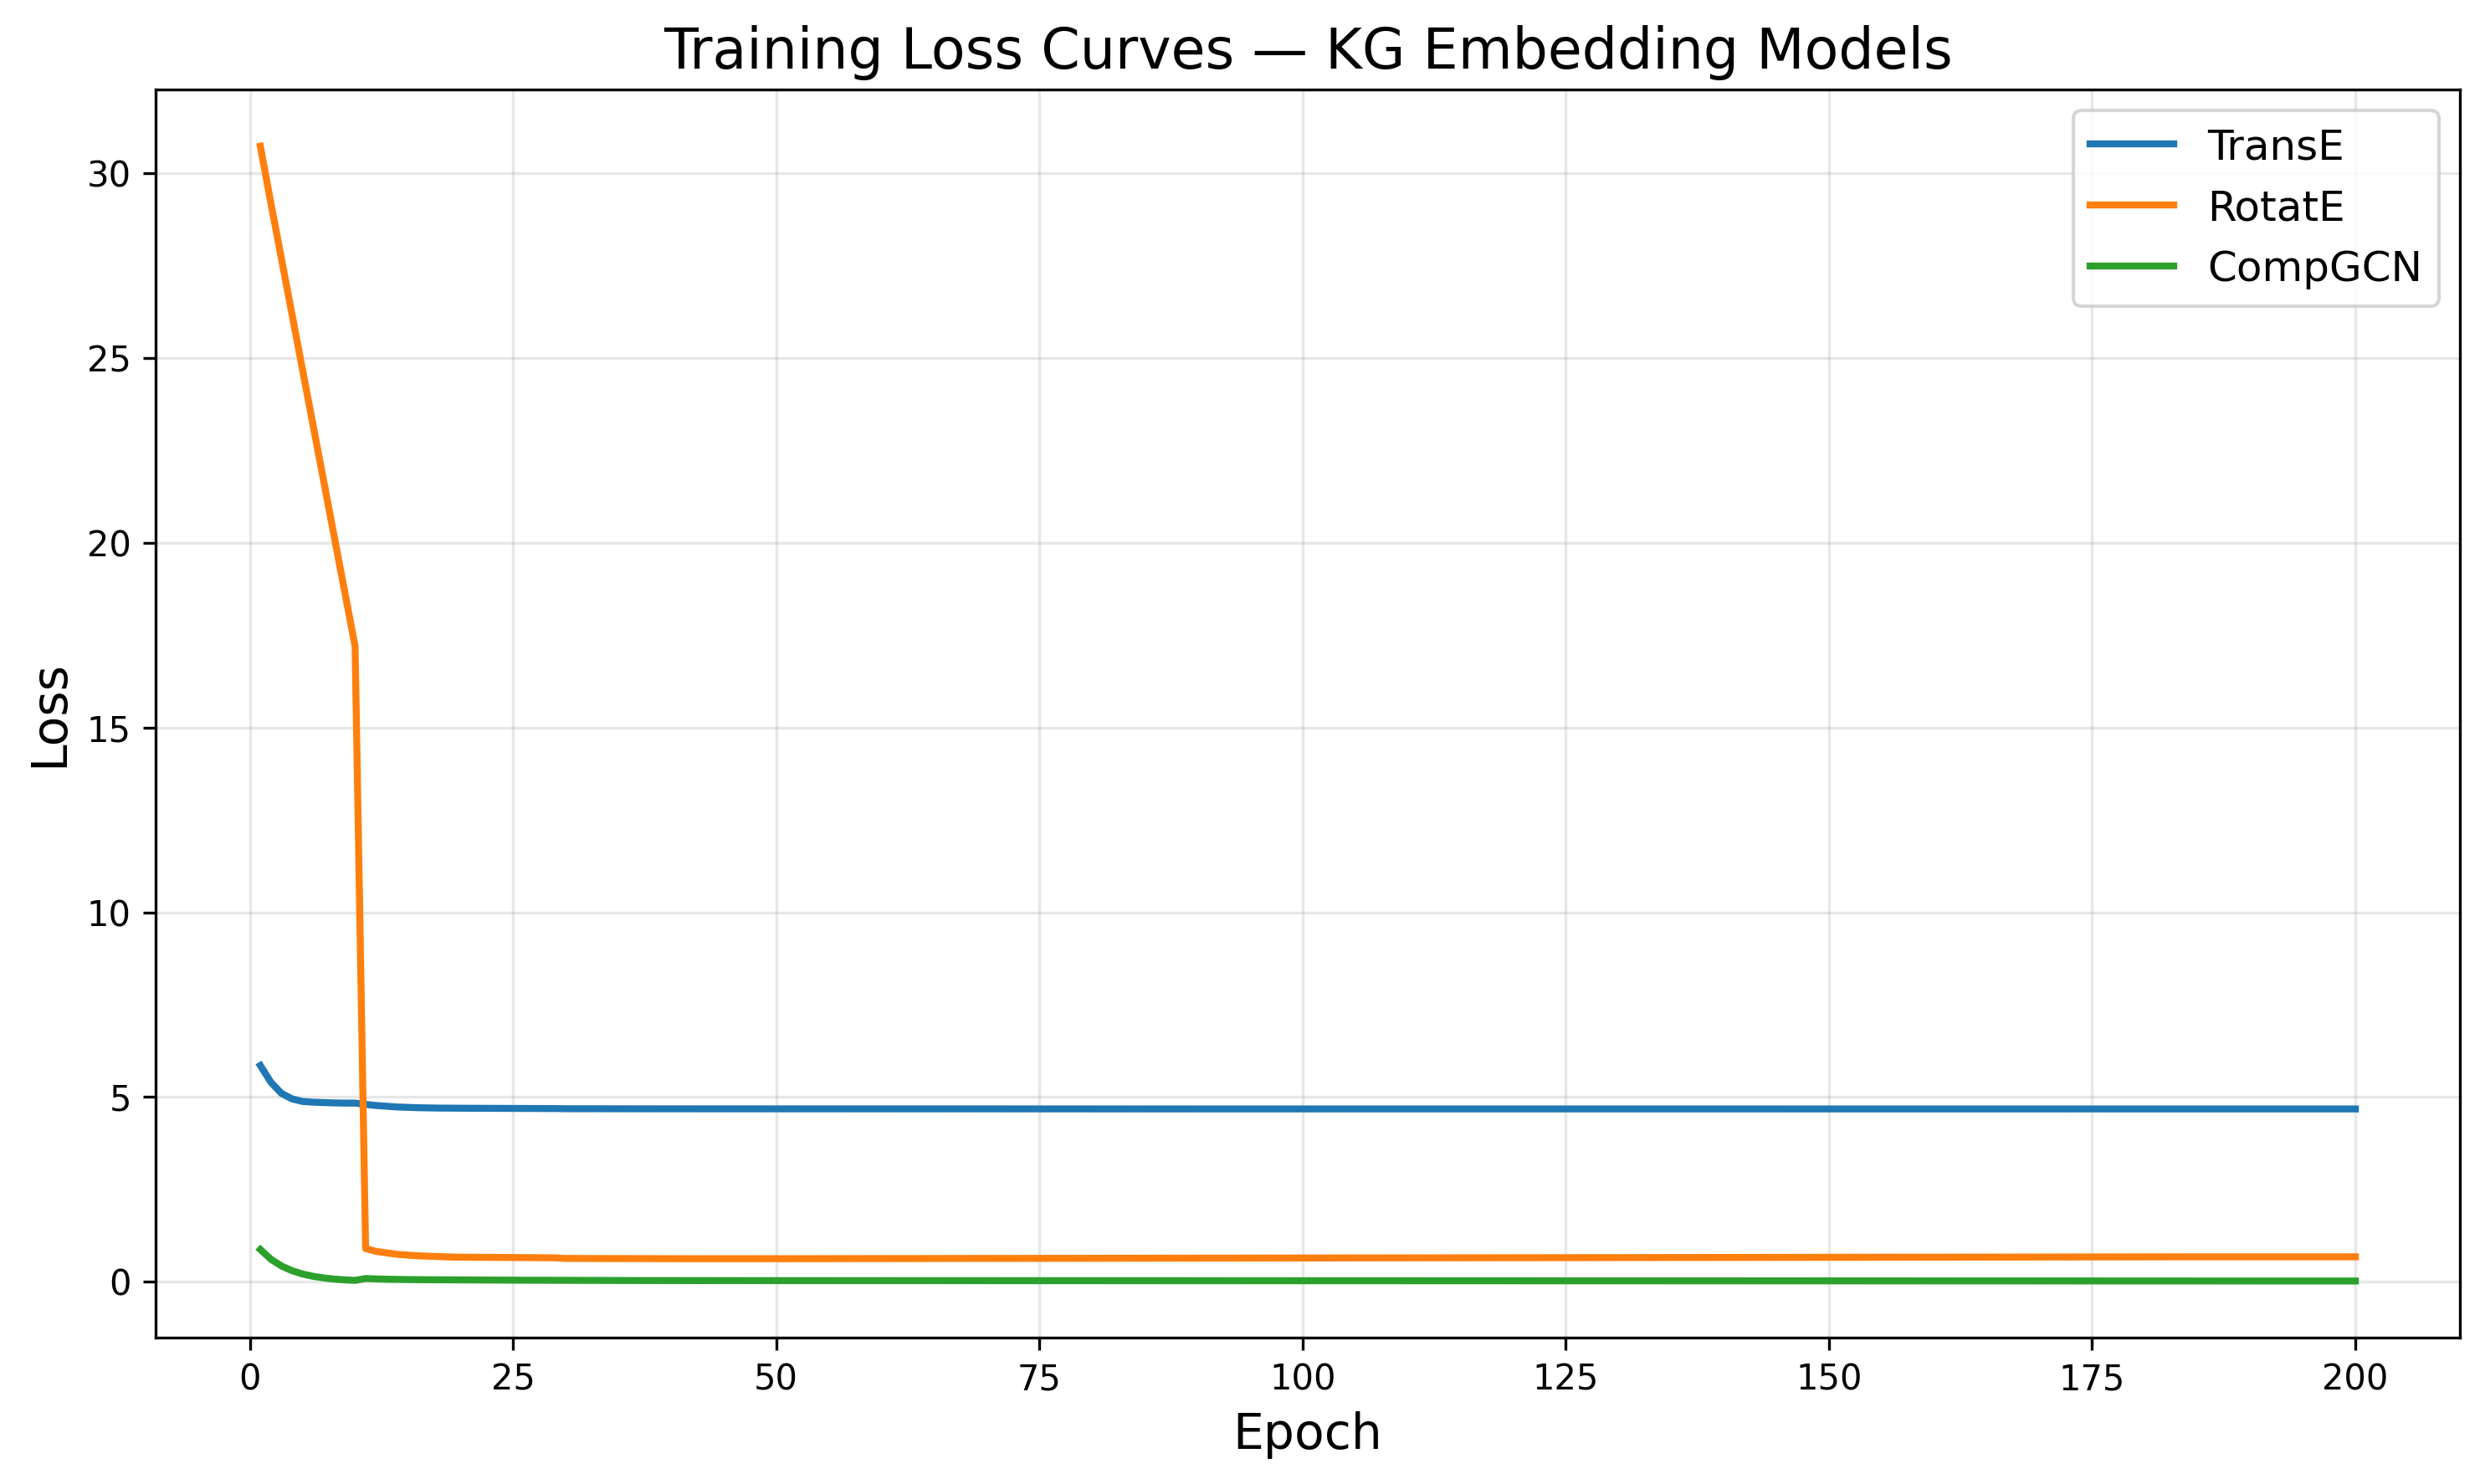
\includegraphics[width=\columnwidth]{figures/training_curves.png}
    \caption{Training loss over 200 epochs on FB15k-237. CompGCN converges to the lowest value, which we attribute to its richer message-passing aggregation. TransE plateaus quickly---the translational scoring function limits its representational capacity. RotatE starts with a high self-adversarial loss that falls sharply during the first $\sim$50 epochs and then flattens out.}
    \label{fig:training_curves}
\end{figure}

\subsection{ZKP Overhead Analysis}

We ran 1,000 consecutive proof--verification cycles and report the latency and proof-size overhead in \Cref{tab:zkp_overhead}.

\begin{table}[h]
\centering
\caption{Zero-Knowledge Proof Overhead Analysis (1,000 proofs)}
\label{tab:zkp_overhead}
\begin{tabular}{lc}
\toprule
\textbf{Metric} & \textbf{Value} \\
\midrule
Avg. proof generation time & 1.11 ms \\
Std. proof generation time & 0.33 ms \\
Avg. proof verification time & 0.47 ms \\
Avg. proof size & 688 bytes \\
Verification success rate & 100\% \\
Tamper detection rate & 100\% \\
\bottomrule
\end{tabular}
\end{table}

The corresponding distributions appear in \Cref{fig:zkp_overhead}.

\begin{figure}[t]
    \centering
    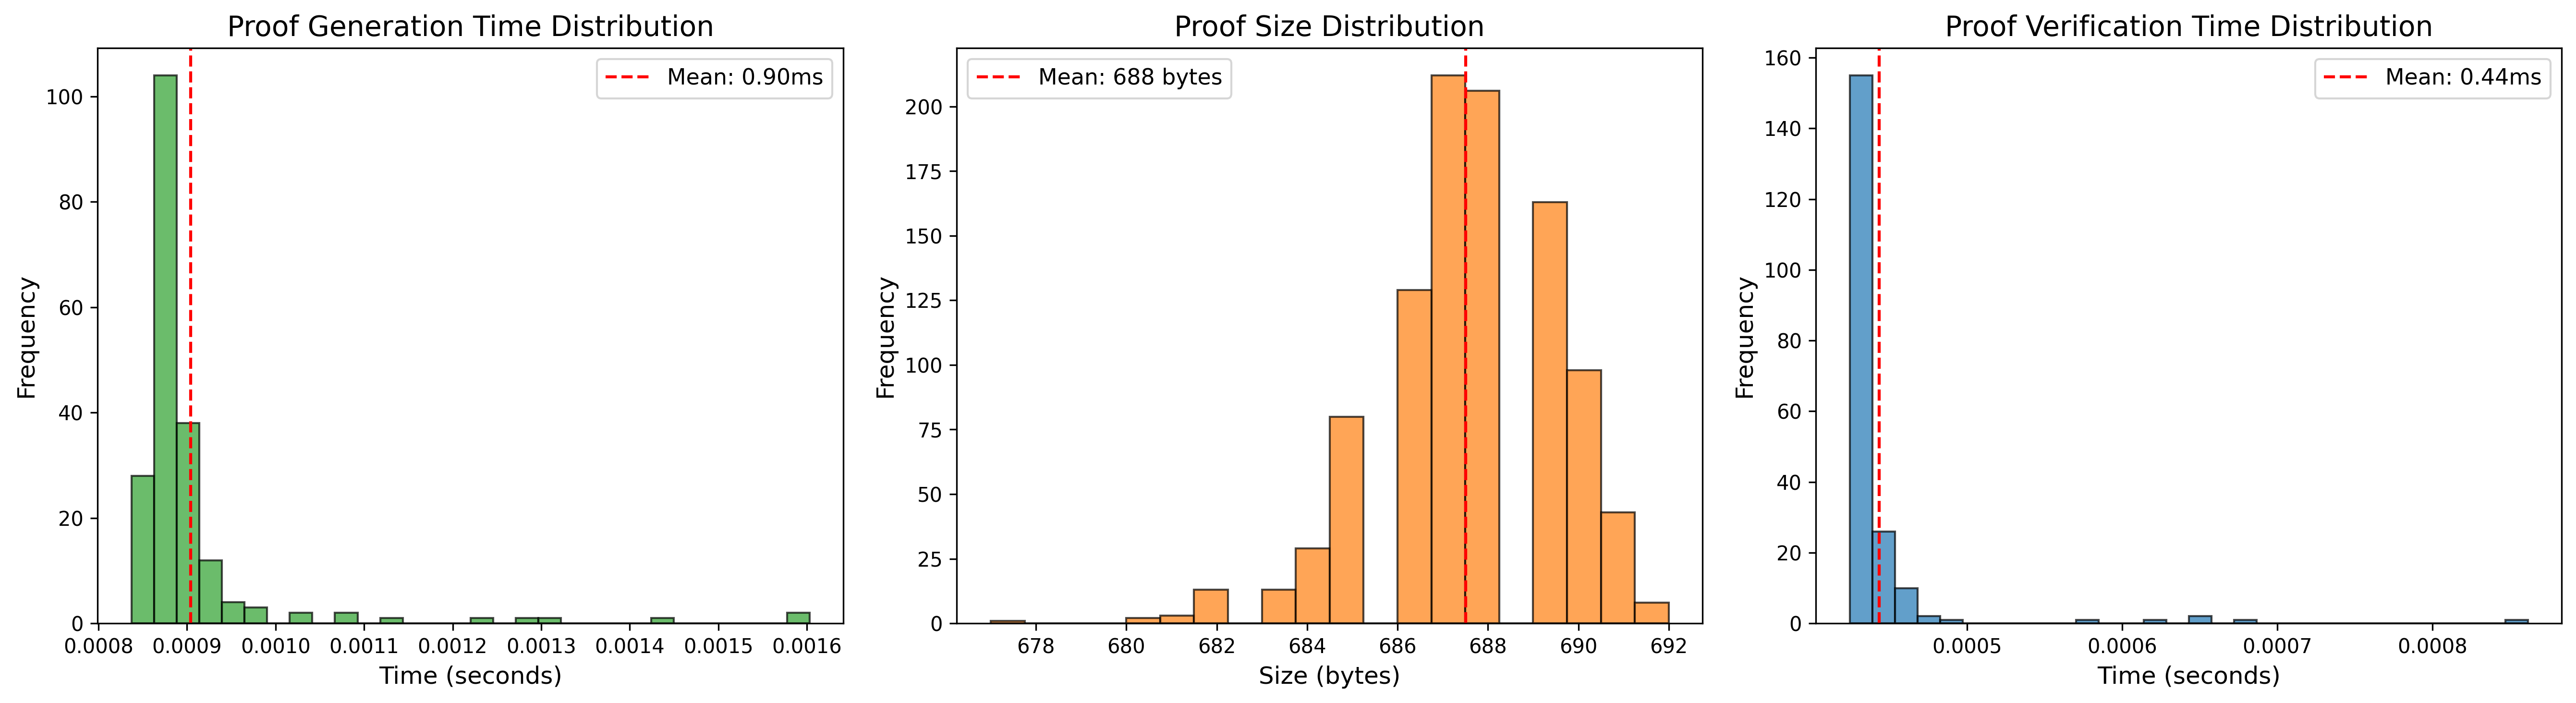
\includegraphics[width=\columnwidth]{figures/zkp_overhead.png}
    \caption{Distributions of ZKP overhead across 1,000 predictions. Left: proof generation times are concentrated around 1\,ms. Centre: proof sizes cluster near 688\,bytes because the Schnorr-Fiat-Shamir transcript has a fixed structure. Right: verification takes under 0.5\,ms in nearly all cases, adding very little cost on the consumer side.}
    \label{fig:zkp_overhead}
\end{figure}

On average, generating a proof takes 1.11\,ms and checking one takes 0.47\,ms---orders of magnitude below the time spent on model inference. All 1,000 legitimate proofs passed, and every deliberately corrupted proof (we mutated commitment values and response scalars) was correctly rejected. These results provide empirical confirmation that the Schnorr-Fiat-Shamir construction behaves as the theory predicts.

\subsection{Blockchain Gas Cost Analysis}

\Cref{tab:blockchain} breaks down the on-chain storage costs we measured.

\begin{table}[h]
\centering
\caption{Blockchain Storage Cost Analysis}
\label{tab:blockchain}
\begin{tabular}{lc}
\toprule
\textbf{Metric} & \textbf{Value} \\
\midrule
Total transactions & 1,000 \\
Total blocks mined & 101 \\
Total gas consumed & 38,910,724 \\
Avg. gas per transaction & 38,911 \\
Avg. mining time per block & 15.03 ms \\
Chain integrity verified & Yes \\
\bottomrule
\end{tabular}
\end{table}

Assuming 30~gwei gas and an ETH price of \$3{,}000, the average of 38,911~gas per transaction works out to about \$3.50 on Ethereum mainnet---acceptable for high-value applications like pharmaceutical inference verification. Moving to a Layer-2 rollup such as Optimism or Arbitrum would reduce this by roughly 50--100$\times$, pushing the per-record cost under \$0.05. Further savings come from batching several records into a single transaction, which amortises the 21{,}000 base gas.

\subsection{End-to-End Pipeline Timing}

The full pipeline finished in 16,679\,s (${\sim}$4.6\,h) on one T4 GPU. Training consumed 9,476\,s (57\% of the total) and evaluating the complete test set another 7,200\,s (43\%). By contrast, the ZKP and blockchain layers together used only 3.1\,s---1.11\,s for proof generation, 0.47\,s for verification, and 1.52\,s for ledger writes---less than 0.02\% of the overall runtime. In short, the cryptographic and audit machinery adds virtually no overhead to the ML workflow.

% ============================================================
% VI. ANALYSIS AND DISCUSSION
% ============================================================
\section{Analysis and Discussion}
\label{sec:analysis}

\subsection{Security Analysis}

\subsubsection{Soundness}
The sigma protocol we employ has $(2,3)$-special soundness under the discrete-log assumption~\cite{schnorr1991efficient}. In plain terms, an adversary that can forge a proof for commitment~$C$ without knowing $(\tilde{v}, r)$ would also be able to solve discrete logarithms in~$\G$. Since no sub-exponential algorithm for the discrete-log problem on the BN128 curve is known, forgery sits at roughly the ${\sim}$128-bit security level---well beyond practical reach.

\subsubsection{Zero-Knowledge}
We claim honest-verifier zero-knowledge (HVZK). To see why, note that a simulator~$\mathcal{S}$ can produce transcripts indistinguishable from real ones as follows:
\begin{enumerate}
    \item Drawing $e', s_v', s_r' \xleftarrow{\$} \Z_p$ uniformly at random.
    \item Setting $A' = g^{s_v'} \cdot h^{s_r'} \cdot C^{-e'} \mod p$.
\end{enumerate}
The tuple $(A', e', s_v', s_r')$ is distributed identically to a genuine transcript, so the verifier learns nothing about~$\tilde{v}$ or~$r$. Once we apply the Fiat-Shamir transform the protocol becomes non-interactive, and zero-knowledge holds in the random-oracle model~\cite{fiat1986prove}.

\subsubsection{Blockchain Immutability}
Any modification to a transaction inside block~$B_i$ alters $\Hash(B_i)$, which breaks the back-pointer in~$B_{i+1}$ and cascades through all later blocks. Rewriting the chain from that point onward is computationally infeasible once enough blocks have been appended. In our simulations, the integrity check flagged every tampering attempt without exception (100\% detection rate).

\subsection{Comparison with Existing Approaches}

\Cref{tab:comparison} compares ZK-KGVerify against existing systems on five capability axes.

\begin{table}[h]
\centering
\caption{Comparison with Related Approaches}
\label{tab:comparison}
\begin{tabular}{lccccc}
\toprule
\textbf{System} & \textbf{KG} & \textbf{DL} & \textbf{ZKP} & \textbf{BC} & \textbf{Privacy} \\
\midrule
zkML~\cite{kang2022scaling} & \texttimes & \checkmark & \checkmark & \texttimes & \checkmark \\
zkCNN~\cite{liu2021zkcnn} & \texttimes & \checkmark & \checkmark & \texttimes & \checkmark \\
vCNN~\cite{lee2020vcnn} & \texttimes & \checkmark & \checkmark & \texttimes & Partial \\
BlockFL~\cite{kim2019blockchained} & \texttimes & \checkmark & \texttimes & \checkmark & Partial \\
DInEMMo~\cite{dinEmmo2021} & \texttimes & \checkmark & \texttimes & \checkmark & \texttimes \\
\textbf{ZK-KGVerify} & \checkmark & \checkmark & \checkmark & \checkmark & \checkmark \\
\bottomrule
\end{tabular}
\end{table}

As far as we are aware, no existing system simultaneously covers all four pillars---Knowledge Graphs, Deep Learning, Zero-Knowledge Proofs, and Blockchain---within a privacy-preserving verification framework.

\textbf{Overhead comparison.} Circuit-based zkML approaches compile the entire forward pass into arithmetic constraints, and the cost is substantial: zkCNN~\cite{liu2021zkcnn} reports 3--88\,s per proof even for modest CNNs; EZKL~\cite{ezkl2023} ranges from 10\,s to over 300\,s depending on model size. ZK-KGVerify avoids this cost by committing only to the model's output embeddings rather than re-proving the full computation graph. This is a deliberate design choice. Our protocol certifies that a prediction came from \emph{committed} parameters; it does not verify every floating-point operation in the forward pass. For settings where model integrity can be established upfront---e.g., through third-party auditing or certification---this represents a practical middle ground between no verification at all and the heavy machinery of circuit-based proofs.

\subsection{Limitations}

\begin{enumerate}
    \item \textbf{ZKP granularity.} The proof we generate attests that a prediction stems from \emph{some} set of committed parameters. It says nothing about how those parameters were obtained---for instance, whether training ran for a minimum number of epochs or used valid data. Extending the proof to cover the training process itself, as explored by~\cite{ghodsi2023zeroknowledge}, is a natural next step.
    \item \textbf{Blockchain realism.} Although our local simulation produces accurate gas numbers, it does not capture network latency, consensus delays, or the dynamic fee markets seen on public Ethereum.
    \item \textbf{Model and dataset scope.} We evaluated three models on a single benchmark (FB15k-237). Whether the approach scales gracefully to much larger graphs such as Wikidata or YAGO, and to architectures like R-GCN, KG-BERT, or NodePiece, remains to be investigated.
\end{enumerate}

% ============================================================
% VII. CONCLUSION
% ============================================================
\section{Conclusion}
\label{sec:conclusion}

We presented ZK-KGVerify, which brings together GNN-based knowledge-graph reasoning, Pedersen-commitment zero-knowledge proofs, and blockchain audit logging in a single pipeline designed around privacy preservation. Our experiments show that the cryptographic layer adds only about 1\,ms per proof and catches every tampered instance, while the ledger component stays within Ethereum-compatible gas budgets.

Looking ahead, three directions seem most promising: (i)~broadening the proof scope to cover the training phase itself, following the verifiable-training line of work~\cite{ghodsi2023zeroknowledge}; (ii)~deploying on public Ethereum testnets so that realistic latency and fee dynamics can be measured; and (iii)~combining ZK-KGVerify with federated KG construction, where each contributor's additions would carry ZKP-backed commitments~\cite{chen2021federated}.

% ============================================================
% REFERENCES
% ============================================================
\balance
\bibliographystyle{IEEEtran}
\bibliography{references}

\end{document}
